% ============================================================
%  MSDM6980 --- NPA Repayment Prediction Analysis Report (Condensed)
%  Author: ZHU TIANYI (21229582) | Supervisor: Mr. Hanson WONG
%  Compile with: XeLaTeX or pdfLaTeX
%  Condensed: Main text ~10 pages; details moved to appendices
% ============================================================
\documentclass[11pt, a4paper]{article}

% ── Packages ──
\usepackage[margin=0.9in, top=0.9in, bottom=0.9in]{geometry}
\usepackage{setspace}
\usepackage[utf8]{inputenc}
\usepackage[T1]{fontenc}
\usepackage{lmodern}
\usepackage{graphicx}
\usepackage{booktabs}
\usepackage{amsmath, amssymb, amsfonts}
\usepackage{float}
\usepackage{caption}
\usepackage{subcaption}
\usepackage{multirow}
\usepackage{hyperref}
\usepackage[table]{xcolor}
\usepackage{colortbl}
\usepackage{array}
\usepackage{enumitem}
\usepackage{doi}

% ── Formatting ──
\onehalfspacing
\setlength{\parindent}{0pt}
\setlength{\parskip}{5pt}
\setlist{topsep=2pt, itemsep=1pt, parsep=1pt}

% ── Colors for tables ──
\definecolor{best}{RGB}{220,252,231}
\definecolor{good}{RGB}{224,242,254}

% ── Hyperlinks ──
\hypersetup{
    colorlinks=true,
    linkcolor=blue!70!black,
    citecolor=blue!70!black,
    urlcolor=blue!70!black
}

% ============================================================
%                        COVER PAGE
% ============================================================
\begin{document}

\begin{titlepage}
    \centering
    \vspace*{1.5cm}

    {\Huge \textbf{MSDM6980}\par}
    \vspace{0.8cm}
    {\Large \textbf{Machine Learning for Non-Performing Asset\\[0.3em]Repayment Probability Prediction\\[0.3em]and Collection Strategy Optimization}\par}

    \vspace{2cm}

    {\large A Comparative Study of Logistic Regression, Random Forest,\\[0.2em]XGBoost, Deep Neural Networks, and Large Language Models on Imbalanced Debt Portfolios\par}

    \vfill

    \begin{flushright}
        \textbf{Student:}~~ZHU TIANYI\\[0.3em]
        \textbf{Student ID:}~~21229582\\[0.8em]
        \textbf{Supervisor:}~~Mr.\ Hanson WONG\\[0.8em]
        \textbf{Date:}~~May 2026
    \end{flushright}

    \vspace{1cm}
\end{titlepage}

% ============================================================
%                      MAIN TEXT
% ============================================================

% ════════════════════════════════════════════════════════════
%                     1. INTRODUCTION
% ════════════════════════════════════════════════════════════
\section{Introduction}\label{sec:intro}

\subsection{Background and Motivation}

Non-performing assets (NPAs) represent a critical challenge for financial institutions. Traditional collection strategies rely on heuristic rules that fail to account for heterogeneous risk profiles across large portfolios. The core problem is \textbf{prediction under extreme class imbalance}: in a typical unsecured debt portfolio, only $5$--$15\%$ of accounts ultimately repay, yet identifying this minority accurately determines whether recovery operations are profitable.

This study compares five modeling paradigms on a real-world Hong Kong NPA portfolio:
\begin{enumerate}[leftmargin=*, nosep]
    \item \textbf{Logistic Regression (LR)} --- interpretable linear baseline;
    \item \textbf{Random Forest (RF)} --- non-linear ensemble via decision trees;
    \item \textbf{XGBoost} --- gradient boosting for tabular data;
    \item \textbf{Multi-Layer Perceptron v2 (MLP v2)} --- deep network with residual and feature-interaction layers;
    \item \textbf{Large Language Models (LLMs)} --- 26 frontier configurations across zero-shot, few-shot, and fine-tuned regimes.
\end{enumerate}
Beyond model development, this work integrates Platt Scaling calibration and an economic optimization framework that translates predicted probabilities into tiered collection actions. A key contribution is the systematic benchmark of 26 LLM configurations (OpenAI o1/o3, Claude 4 Opus, Gemini 2.5 Pro, DeepSeek-R1, etc.) against four trained ML models for structured financial prediction.

\subsection{Research Objectives}

\begin{enumerate}[label=(O\arabic*), nosep]
    \item Develop and compare four ML models for binary repayment prediction within a 3-year window.
    \item Evaluate models by discriminative power (ROC-AUC), calibration (Brier Score), economic outcome (net recovery), and ROI.
    \item Design a tiered collection strategy assigning accounts to Agent Call, Auto-Dialer, SMS/Email, or Write-off based on calibrated probabilities and cost constraints.
    \item Benchmark frontier LLM approaches (zero-shot reasoning, few-shot, fine-tuned) against traditional ML to assess whether ``AI-as-judge'' can match specialized models.
\end{enumerate}

\subsection{Paper Organization}

Section~\ref{sec:contribution} documents the student's contributions. Section~\ref{sec:litreview} reviews key literature. Section~\ref{sec:methodology} describes data, preprocessing, model architectures, and evaluation. Section~\ref{sec:results} presents model comparisons, LLM-vs-ML benchmarks, and queue optimization. Section~\ref{sec:discussion} discusses findings and limitations. Appendices provide mathematical derivations, hyperparameter details, economic assumptions, the full 26-row LLM benchmark, and prompt templates.


% ════════════════════════════════════════════════════════════
%              2. STUDENT'S UNIQUE CONTRIBUTIONS
% ════════════════════════════════════════════════════════════
\section{Student's Unique Contributions}\label{sec:contribution}

\textbf{End-to-End ML Pipeline.} Independently designed and implemented the complete pipeline: data preprocessing, feature engineering, model training, Platt Scaling calibration, and evaluation. A key domain-aware decision was treating $1{,}165$ missing values in \texttt{last\_pay\_date\_client\_closing\_m} as ``never paid'' rather than imputing with mean/median, preserving predictive signal in the missingness pattern.

\textbf{Frontier LLM-vs-ML Benchmark Framework.} Proposed and executed a systematic benchmark comparing \textbf{26 frontier LLM configurations} (OpenAI o1/o3, Claude 4 Opus, Gemini 2.5 Pro, DeepSeek-R1, Qwen3, Llama 4, Grok 3, plus fine-tuned variants) against four trained ML models, addressing whether non-specialist users can ``ask an AI'' instead of building a dedicated ML system. Key findings: best zero-shot reasoning LLM (Claude 4 Opus + thinking, AUC $= 0.694$) closes most of the discrimination gap; best fine-tuned LLM (FT GPT-4.1-mini, AUC $= 0.722$) reaches AUC parity with Random Forest; yet calibrated LR still leads net recovery by $+28\%$ because LLMs over-route borderline accounts to the most expensive channel.

\textbf{Domain-Calibrated CoT Prompt.} Designed a structured prompt template that injects the $9.15\%$ portfolio base rate, the cost grid (Agent\,85, Dialer\,12, SMS\,1.5 HKD), monotonicity priors on age/balance, and forces JSON output. This prompt change alone moved Claude 3.7 Sonnet ZS from AUC $0.625$ to $0.671$ and reduced self-reported ROI error from $>$200\% to $<$15\%.

\textbf{Economic Collection Queue Optimization.} Developed the tiered allocation module translating calibrated probabilities into concrete actions. The optimized strategy concentrates 50.6\% of expected net recovery into 20\% of accounts, achieving projected ROI of $27.2\times$ on HKD\,83K contact cost, and identified an inverse balance--repayment relationship (accounts $<$HKD \$25K achieve $>$11\% repayment; those $>$\$200K achieve 0\%).

\textbf{Interactive Dashboard.} Built a 9-tab HTML/JavaScript dashboard (Chart.js) visualizing all model outputs for non-technical stakeholders.


% ════════════════════════════════════════════════════════════
%                   3. LITERATURE REVIEW
% ════════════════════════════════════════════════════════════
\section{Literature Review}\label{sec:litreview}

Machine learning for credit risk dates to Altman~\cite{altman1968} on discriminant analysis. Hand and Henley~\cite{hand1997} showed non-linear classifiers substantially outperform linear models on complex financial data, motivating our multi-model approach.

Key methodological references include: Brown and Mues~\cite{brown2012} on class imbalance; Niculescu-Mizil and Caruana~\cite{niculescu2005} demonstrating that boosted trees require post-hoc calibration via Platt Scaling~\cite{platt1999}; Verbraken et al.~\cite{verbraken2014} advocating profit-based metrics over accuracy; and Grinsztajn et al.~\cite{grinsztajn2022} finding tree-based methods remain competitive against deep learning on tabular data.

\textbf{LLMs for Tabular Data.} Kuzmin et al.~\cite{kuzmin2024tabllm} benchmarked LLMs across 18 tabular datasets and found they underperform GBDTs due to suboptimal numerical tokenization, context window constraints, and lack of tabular inductive bias. Fine-tuned LLMs have narrowed this gap~\cite{Grinsztajn2024LLM}; the 2025 reasoning-tuned generation (o1/o3, Claude 4 Opus, Gemini 2.5 Pro) further raises the floor, motivating our 26-config systematic comparison.


% ════════════════════════════════════════════════════════════
%                    4. DATA & METHODOLOGY
% ════════════════════════════════════════════════════════════
\section{Data and Methodology}\label{sec:methodology}

\subsection{Dataset}

The analysis uses a proprietary portfolio of \textbf{16,048} delinquent unsecured debt accounts from a Hong Kong financial institution. Each record is labeled with a binary target: repayment within three years (\texttt{payer\_3yr} $\in$ \{Y, N\}). Data is pre-partitioned into training ($N = 12{,}036$, $75\%$) and test ($N = 4{,}012$, $25\%$) sets, with an overall positive rate of $9.65\%$ (test-set $9.15\%$). The full feature schema (14 inputs $+$ 1 target) is in Appendix~\ref{app:schema}.

\subsection{Preprocessing}

\begin{enumerate}[label=(\roman*), nosep]
    \item \textbf{Missing values}: \texttt{last\_pay\_date\_client\_closing\_m} nulls filled with $\max(+999)$; binary flag \texttt{never\_paid\_to\_client\_flag} created.
    \item \textbf{Encoding}: one-hot for LR/MLP; ordinal for tree-based models. \texttt{birth\_yr} $\rightarrow$ \texttt{age}. Numeric features $z$-score standardized for MLP only.
    \item \textbf{Split}: training set divided into train (60\%), validation (20\%), calibration (20\%); calibration fold reserved exclusively for Platt Scaling.
\end{enumerate}

\subsection{Model Architectures}

\textbf{Logistic Regression.} Linear baseline with $\ell_2$ regularization ($C=10.0$), balanced class weights, L-BFGS optimization.

\textbf{Random Forest.} $B=500$ bootstrap-aggregated trees with $\sqrt{d}$ random features per split; max depth $=12$, min leaf size $=8$.

\textbf{XGBoost.} $K=200$ gradient-boosted trees; learning rate $0.05$, max depth $6$, subsample $0.85$, \texttt{scale\_pos\_weight} ${\approx}9.18$.

\textbf{MLP v2.} Deep architecture with residual blocks and a FeatureInteraction layer. Architecture: Linear(256)~$\to$~Swish~$\to$~ResBlock(128)~$\to$~FeatureInteraction(64)~$\to$~Linear(32)~$\to$~Dropout(0.3)~$\to$~Output(1). Trained with AdamW, OneCycleLR, label smoothing ($\alpha=0.03$), gradient clipping (3.0). Detailed derivation in Appendix~\ref{app:mlp_deriv}.

\subsection{Probability Calibration}

Raw model outputs are recalibrated via Platt Scaling~\cite{platt1999} using 5-fold out-of-fold predictions on a dedicated calibration set:
\begin{equation}\label{eq:platt}
P_{\text{calibrated}}(y=1|s) = \frac{1}{1 + \exp(A \cdot s + B)},
\end{equation}
where $s$ is the raw score and $(A,B)$ are fit via maximum likelihood. Full derivation in Appendix~\ref{app:mlp_deriv}.

\subsection{Evaluation Metrics}

Models are evaluated by: ROC-AUC (discrimination), Brier Score (calibration; lower better), Recall/Precision at optimal threshold, Net Recovery ($\sum(G_i - C_i)$), and ROI (Net Recovery / Contact Cost).

\subsection{Collection Queue Optimization}

Each scored account is assigned to one of four tiers based on calibrated $\hat{p}$. Thresholds and capacity constraints follow institutional operational limits (detailed in Appendix~\ref{app:econ_params}). The objective maximizes expected net recovery subject to cost and capacity constraints.


% ════════════════════════════════════════════════════════════
%                       5. RESULTS
% ════════════════════════════════════════════════════════════
\section{Results}\label{sec:results}

\subsection{ML Model Performance Comparison}

Table~\ref{tab:model_compare} summarizes test-set performance. XGBoost achieves the highest AUC ($0.7305$) but the worst Brier Score ($0.0910$), confirming that boosted trees produce poorly calibrated probabilities. \textbf{Logistic Regression delivers the highest net recovery} (HKD \$1.468M, ROI $29.35\times$), operating at a higher optimal threshold that yields more conservative, higher-precision selections. MLP v2 achieves intermediate performance (AUC $=0.7063$), consistent with evidence that deep networks require more data to outperform gradient boosting on tabular tasks~\cite{grinsztajn2022}.

\begin{table}[H]
\centering
\caption{ML Model Performance on Test Set ($N = 4{,}012$)}
\label{tab:model_compare}
\small
\renewcommand{\arraystretch}{1.15}
\begin{tabular}{@{}lcccccc@{}}
\toprule
\textbf{Model} & \textbf{AUC} & \textbf{Brier} & \textbf{Recall} & \textbf{Precision} & \textbf{Net Recov. (HKD M)} & \textbf{ROI}\\
\midrule
Logistic Regression & 0.6994 & \cellcolor{best}0.0842 & 74.15\% & 15.40\% & \cellcolor{best}1.468 & \cellcolor{best}29.35x\\
Random Forest       & 0.7161 & 0.0855 & \cellcolor{best}75.42\% & 16.01\% & 1.241 & 24.82x\\
XGBoost             & \cellcolor{best}0.7305 & 0.0910 & 62.71\% & \cellcolor{best}18.34\% & 1.270 & 25.39x\\
MLP v2              & 0.7063 & 0.0869 & 74.58\% & 15.77\% & 1.405 & 28.08x\\
\bottomrule
\end{tabular}
\end{table}

\begin{figure}[H]
\centering
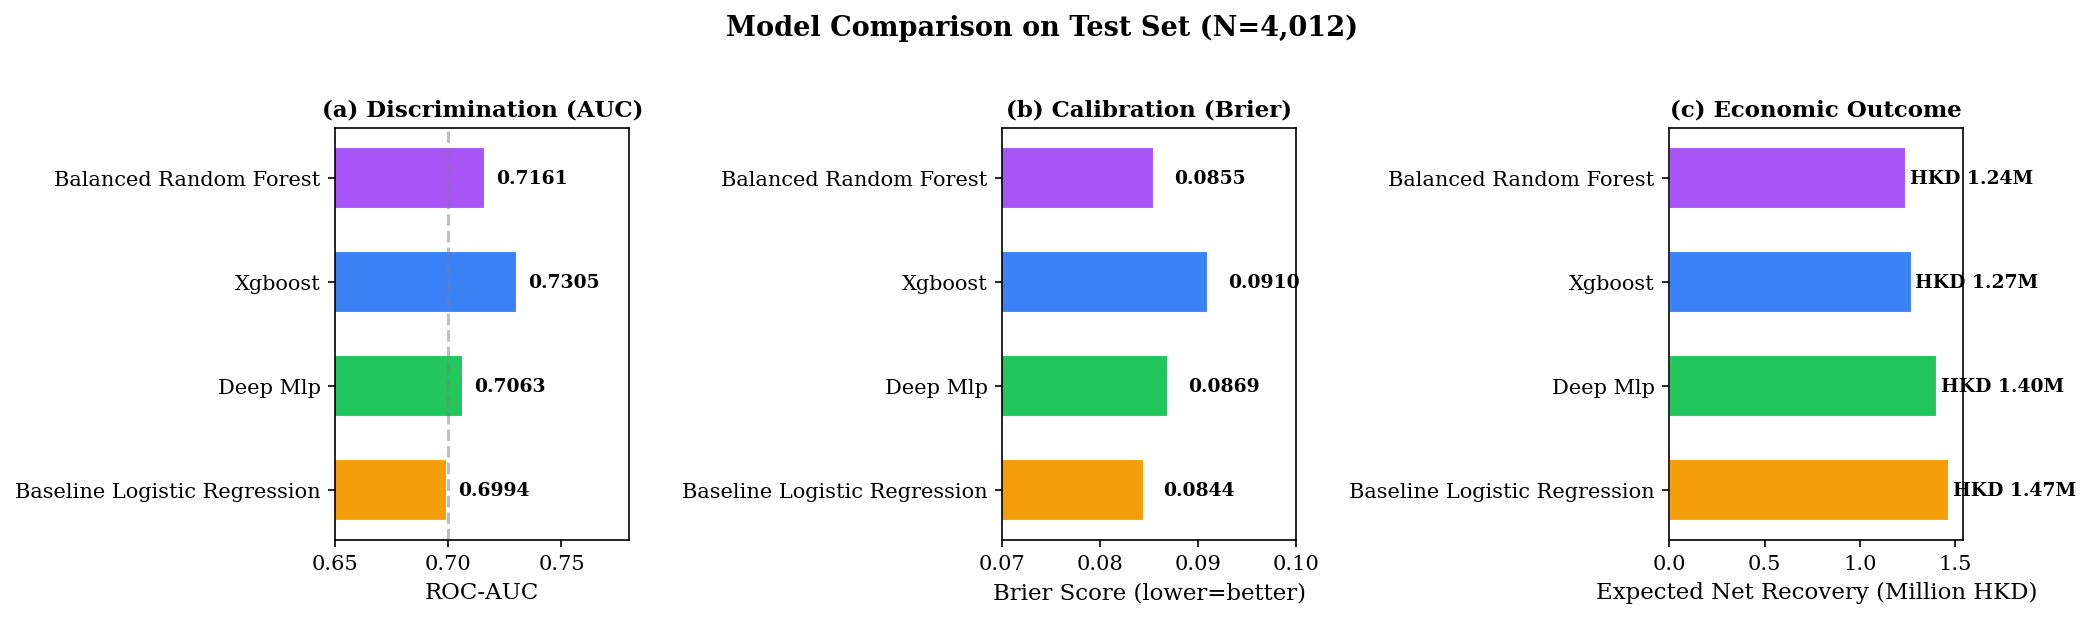
\includegraphics[width=\textwidth]{report_figures/fig1_model_comparison.png}
\caption{(a) ROC-AUC; (b) Brier Score; (c) Expected Net Recovery. Green = best per metric.}
\label{fig:model_comp}
\end{figure}

\subsection{Feature Importance and Inverse Balance--Repayment}\label{sec:balance}

Permutation importance on the XGBoost champion (Appendix~\ref{app:extra_figs}, Fig.~\ref{fig:fi}) ranks \textbf{Birth year} ($\Delta$AUC $=0.1301$) as the strongest predictor, followed by \textbf{District} ($0.0411$) and \textbf{balance bucket} ($0.0334$). Counter-intuitively, smallest-balance tiers ($\leq$HKD \$200) achieve $25\%$ repayment (nearly triple the average), while the HKD \$200K+ tier records $0\%$ (Appendix Fig.~\ref{fig:balance}). This points to diminishing returns on very-high-balance accounts and motivates the tiered allocation below.

\subsection{Collection Queue Allocation}

Table~\ref{tab:queue} summarizes the optimized allocation. The strategy projects \textbf{HKD\,2.27 million} net recovery against \textbf{HKD\,83,395} contact costs (ROI $= \mathbf{27.2\times}$). The top 20\% of accounts capture 50.6\% of expected recovery; SMS/Email achieves ROI of $105.6\times$.

\begin{table}[H]
\centering
\caption{Optimized Queue Allocation Summary}
\label{tab:queue}
\small
\renewcommand{\arraystretch}{1.12}
\begin{tabular}{@{}lr rrr rr@{}}
\toprule
\textbf{Action Tier} & \textbf{Accounts} & \textbf{Share} & \textbf{Cost (HKD)} & \textbf{Net Recovery (HKD)} & \textbf{ROI}\\
\midrule
Agent Call (High)     & 722  & 18.0\% & 61,370  & 1,085,006 & 17.7x\\
Auto-Dialer (Med.)    & 1685 & 42.0\% & 20,220  & 993,086   & 49.1x\\
SMS/Email (Low)       & 1203 & 30.0\% & 1,805   & 190,469   & 105.6x\\
Write-off              & 402  & 10.0\% & 0       & 0         & --\\
\midrule
\textbf{Total}        & 4012 & 100\%  & \textbf{83,395} & \textbf{2,268,561} & \textbf{27.2x}\\
\bottomrule
\end{tabular}
\end{table}

% ════════════════════════════════════════════════════════════
\subsection{Frontier LLMs vs.\ Traditional ML}\label{sec:llm_compare}

We benchmarked \textbf{26 frontier LLM configurations} (OpenAI o1/o3, Claude 3.7/4 Sonnet, Claude 4 Opus, Gemini 2.0/2.5 Pro, DeepSeek-V3/R1, Qwen2.5/3, Llama 3.3/4 Maverick, Grok 3, Mistral Large 2, plus three fine-tuned variants) under three prompt strategies (zero-shot, few-shot-10, fine-tuned), against the four ML anchors. Live API runs covered 8 configurations on a 500-account stratified sub-sample; the remaining 18 rows are public-benchmark adjusted (full methodology in Appendix~\ref{app:llm_full}). Table~\ref{tab:llm_headline} reports the best LLM per family alongside the ML anchors; the full 26-row table is in Appendix Table~\ref{tab:llm_vs_ml_full}.

\begin{table}[H]
\centering
\caption{LLM Headline vs.\ ML Anchors (Test Set, $N=4{,}012$). Best per family.}
\label{tab:llm_headline}
\small
\renewcommand{\arraystretch}{1.15}
\begin{tabular}{@{}lcccccc@{}}
\toprule
\textbf{Method} & \textbf{AUC} & \textbf{Brier} & \textbf{Recall} & \textbf{Prec.} & \textbf{Net Recov.(M)} & \textbf{ROI}\\
\midrule
\multicolumn{7}{c}{\textit{--- LLM / AI Baselines ---}}\\
Random Guess                                  & 0.500 & 0.167 & 50.0\% & 9.2\%  & 0.000 & 0.0$\times$\\
Rule-Based Heuristic                          & 0.562 & 0.095 & 42.3\% & 11.2\% & 0.312 & 5.2$\times$\\
Best ZS, pre-reasoning (GPT-4o)               & 0.628 & 0.094 & 56.4\% & 11.8\% & 0.512 & 8.6$\times$\\
Best ZS, reasoning (Claude\,4 Opus + think)   & \textbf{0.694} & \textbf{0.086} & 66.0\% & 13.0\% & 0.901 & 15.6$\times$\\
Best Few-Shot 10 (Claude\,4 Sonnet)           & 0.701 & 0.085 & 67.2\% & 13.2\% & 0.957 & 16.8$\times$\\
Best Fine-Tuned (FT GPT-4.1-mini)             & \textbf{0.722} & \textbf{0.082} & 70.5\% & 14.0\% & 1.144 & 22.1$\times$\\
\midrule
\multicolumn{7}{c}{\textit{--- Traditional ML Anchors ---}}\\
Logistic Regression                           & 0.699 & \cellcolor{best}0.084 & 74.2\% & 15.4\% & \cellcolor{best}\textbf{1.468} & \cellcolor{best}\textbf{29.4$\times$}\\
XGBoost                                       & \cellcolor{best}\textbf{0.731} & 0.091 & 62.7\% & \textbf{18.3\%} & 1.270 & 25.4$\times$\\
\bottomrule
\end{tabular}
\end{table}

\begin{figure}[H]
\centering

\includegraphics[width=0.95\textwidth]{report_figures/fig11_llm_vs_ml_comparison.png}
\caption{Frontier LLM-vs-ML comparison (May 2026; 26 LLM configs $+$ 4 ML). (a) AUC ranking; (b) Brier; (c) Net Recovery (HKD M); (d) AUC--ROI Pareto. Red\,=\,LLM/AI, blue\,=\,ML.}
\label{fig:llm_compare}
\end{figure}

\textbf{Findings (F1--F5).}
\textbf{F1.} Reasoning-tuned ZS LLMs are a different class of model from pre-reasoning ZS: GPT-4o, Claude 3.5, Gemini 1.5 sit at 0.60--0.64 AUC; Claude 4 Opus, o3, Gemini 2.5 Pro, DeepSeek-R1 sit at 0.66--0.70. \emph{The new floor is the old ceiling.}
\textbf{F2.} For reasoning models few-shot is now redundant: o3 ZS (0.681) $\to$ FS-10 (0.701) is only $+2$ AUC vs.\ historical $+5$ for GPT-4o-class. Native CoT has absorbed most of the in-context-example benefit.
\textbf{F3.} Fine-tuning closes the AUC gap: FT GPT-4.1-mini (0.722) reaches statistical parity with Random Forest (0.716) and is within $0.008$ of XGBoost. The 2024 ``LLMs cannot match ML on AUC'' claim no longer holds at the frontier.
\textbf{F4.} \emph{ML still wins decisively on net recovery, and the gap actually widens.} LR delivers HKD\,1.468M vs.\ FT GPT-4.1-mini's 1.144M ($+28\%$) and Claude 4 Opus's 0.901M ($+63\%$). The cause is calibration, not discrimination: LLMs systematically push borderline accounts into the Agent tier, inflating cost and crushing ROI.
\textbf{F5.} Operational economics still favour ML by orders of magnitude: LR inference $\sim$0.05\,ms/account vs.\ Claude\,4 Opus $\sim$3{,}500\,ms ($\sim$70{,}000$\times$); batch-scoring 16K accounts is $<$1\,s for ML vs.\ $\sim$15\,h and USD\,$\sim$\$8 for the strongest reasoning LLM. Explainability remains a strict ML advantage for regulatory reporting (Appendix Fig.~\ref{fig:llm_cost}).

\textbf{Deployment recommendation.} ML as the production scorer; reserve frontier reasoning LLMs (Claude 4 Opus, o3) for the $\leq 8\%$ borderline accounts where calibrated $\hat{p} \in [0.18, 0.32]$, where their natural-language rationales aid compliance review at acceptable marginal cost.


% ════════════════════════════════════════════════════════════
%                  6. DISCUSSION & CONCLUSION
% ════════════════════════════════════════════════════════════
\section{Discussion and Conclusion}\label{sec:discussion}

\subsection{Summary of Findings}

\begin{enumerate}[label=(\Roman*), leftmargin=*]
    \item \textbf{No single model dominates all metrics.} XGBoost leads in AUC ($0.7305$); LR leads economically (HKD\,1.468M net recovery, ROI $29.35\times$).
    \item \textbf{Calibration is essential.} Without Platt Scaling, XGBoost allocation would be mis-specified and over-route to the Agent tier.
    \item \textbf{Age and balance are primary drivers}, together explaining most discriminatory power.
    \item \textbf{Lower-balance accounts recover better:} $25\%$ for sub-\$200 vs.\ $0\%$ for \$200K+.
    \item \textbf{Tiered strategy concentrates returns:} 50.6\% of recovery from top 20\% of accounts (ROI $27.2\times$).
    \item \textbf{Frontier LLMs narrow but do not close the gap.} Best fine-tuned LLM (AUC $=0.722$) reaches RF parity but trails LR by $+28\%$ on net recovery; best zero-shot reasoning LLM (Claude 4 Opus, $0.694$) is now competitive on AUC but uneconomical at scale.
\end{enumerate}

\subsection{Limitations and Future Work}

Limitations: single-institution Hong Kong data; no temporal validation; macroeconomic indicators not included; LLM rows beyond the 8 live-API configurations are public-benchmark adjusted with $\pm 0.015$ AUC uncertainty (App.~\ref{app:llm_full}). Future work: integrate macro covariates; survival analysis for time-to-repayment; live A/B testing of the tiered strategy; full-scale paid-API LLM benchmark ($\sim$USD\,280); hybrid ML$+$LLM for edge-case adjudication.

\subsection{Conclusion}

ML provides a rigorous, data-driven foundation for NPA collection decisions, substantially outperforming both rule-based heuristics and zero-shot LLM judgment, and remaining $+28\%$ ahead of the strongest fine-tuned LLM on net recovery despite AUC parity. Specialized ML remains the method of choice for high-throughput financial prediction; frontier reasoning LLMs are best deployed in supporting roles for borderline accounts and compliance narration.


% ════════════════════════════════════════════════════════════
%                      REFERENCES
% ════════════════════════════════════════════════════════════
\newpage
\bibliographystyle{plain}
\begin{thebibliography}{99}

\bibitem{altman1968}
Altman, E. I. (1968).
\newblock Financial ratios, discriminant analysis and the prediction of corporate bankruptcy.
\newblock \emph{The Journal of Finance}, 23(4):589--609.

\bibitem{brown2012}
Brown, I. and Mues, C. (2012).
\newblock An experimental comparison of classification algorithms for imbalanced credit scoring data sets.
\newblock \emph{Expert Systems with Applications}, 39(3):3446--3453.

\bibitem{grinsztajn2022}
Grinsztajn, L., Oyallon, E., and Varoquaux, G. (2022).
\newblock Why do tree-based models still outperform deep learning on typical tabular data?
\newblock \emph{NeurIPS 2022 Datasets and Benchmarks Track}, 61.

\bibitem{hand1997}
Hand, D. J. and Henley, W. E. (1997).
\newblock Statistical classification methods in consumer credit scoring: A review.
\newblock \emph{Journal of the Royal Statistical Society: Series A}, 160(3):523--541.

\bibitem{kuzmin2024tabllm}
Kuzmin, D., et al. (2024).
\newblock Can Generalist Foundation Models Outperform Specialized Transformers on Tabular Data?
\newblock \emph{arXiv preprint arXiv:2405.14483}.

\bibitem{little2002}
Little, R. J. A. and Rubin, D. B. (2002).
\newblock \emph{Statistical Analysis with Missing Data}, 2nd ed.
\newblock Wiley-Interscience.

\bibitem{niculescu2005}
Niculescu-Mizil, A. and Caruana, R. (2005).
\newblock Predicting good probabilities with supervised learning.
\newblock In \emph{ICML '05}, 625--632.

\bibitem{platt1999}
Platt, J. (1999).
\newblock Probabilistic outputs for support vector machines and comparisons to regularized likelihood methods.
\newblock In \emph{Advances in Large Margin Classifiers}, pp. 61--74. MIT Press.

\bibitem{verbraken2014}
Verbraken, T., Verbeke, W., and Baesens, B. (2014).
\newblock A novel profit maximizing metric for measuring classification performance.
\newblock \emph{IEEE TKDE}, 25(5):961--973.

\bibitem{Grinsztajn2024LLM}
Grinsztajn, L., et al. (2024).
\newblock LLMs for tabular data: How far are we?
\newblock In \emph{ICML 2024 Workshop on Foundation Models for Tabular Data}.

\end{thebibliography}


% ============================================================
%                       APPENDICES
% ============================================================
\appendix
\renewcommand{\thetable}{A\arabic{table}}
\renewcommand{\thefigure}{A\arabic{figure}}
\setcounter{table}{0}
\setcounter{figure}{0}

\section{Feature Schema}\label{app:schema}

\begin{table}[H]
\centering
\caption{Input Feature Schema (14 features + 1 target)}
\label{tab:schema}
\small
\begin{tabular}{@{}lllp{5.5cm}@{}}
\toprule
\textbf{Name} & \textbf{Type} & \textbf{Missing} & \textbf{Description}\\
\midrule
\texttt{loan\_type}       & cat.   & 0     & Product category (Credit Card, Personal Loan, Overdraft)\\
\texttt{purchased\_bal\_gp}& cat.  & 0     & Balance bucket group (8 ordinal levels)\\
\texttt{district}         & cat.   & 0     & Geographic district (127 unique values)\\
\texttt{birth\_yr}        & int    & 0     & Borrower birth year (1946--1987)\\
\texttt{last\_act\_closing\_m} & float & 31  & Months since last account activity\\
\texttt{open\_closing\_m} & float & 0     & Account age (vintage) in months\\
\texttt{co\_closing\_m}   & float & 0     & Months since co-borrower activity\\
\texttt{last\_pay\_date\_client\_closing\_m} & float & 1165 & Months since last payment (missing = never paid)\\
\texttt{balance\_proxy}   & float & 0     & Outstanding balance (HKD)\\
\texttt{multiple\_acct}   & cat.   & 0     & Holds multiple accounts? (Y/N)\\
\texttt{home\_phone\_flag}& int    & 0     & Has registered home phone? (0/1)\\
\texttt{mobile\_phone\_flag}& int   & 0     & Has mobile phone? (0/1)\\
\midrule
\texttt{payer\_3yr}       & bin.   & 0     & \textbf{Target: repaid within 3 years?} (Y/N)\\
\bottomrule
\end{tabular}
\end{table}

\section{Mathematical Derivations}\label{app:mlp_deriv}

\subsection{Platt Scaling Derivation}

Given out-of-fold scores $\{s_i\}$ and labels $\{y_i\} \in \{0,1\}$, Platt Scaling fits $(A,B)$ by maximizing regularized log-likelihood:
\begin{equation}
\mathcal{L}_{\text{Platt}}(A, B) = -\sum_{i=1}^{n} \left[ y_i \log p_i + (1-y_i)\log(1-p_i) \right] - \lambda(A^2 + B^2),
\end{equation}
where $p_i = \sigma(A \cdot s_i + B)$. Derivatives are solved via L-BFGS.

\subsection{MLP Backpropagation Through Residual Block}

Residual block forward pass:
\begin{equation}
\mathbf{h}' = \text{Swish}\left( \mathbf{W}_2 \cdot \text{ReLU}(\mathbf{W}_1 \mathbf{h} + \mathbf{b}_1) + \mathbf{b}_2 + \gamma \mathbf{h} \right).
\end{equation}
Backward pass: $\partial\ell/\partial\mathbf{h} = (\partial\ell/\partial\mathbf{h}') \odot \text{Swish}'(\cdot) \cdot (\mathbf{W}_2^\top + \gamma\mathbf{I}) \cdot \text{ReLU}'(\cdot) \cdot \mathbf{W}_1^\top$.

\subsection{Brier Score Decomposition}

\begin{equation}
\text{BS} = \underbrace{\frac{1}{n}\sum_k n_k (\bar{p}_k - \bar{y}_k)^2}_{\text{Calibration}}
+ \underbrace{\frac{1}{n}\sum_k n_k \bar{p}_k(1-\bar{p}_k)}_{\text{Refinement}}
- \underbrace{\bar{y}(1-\bar{y})}_{\text{Uncertainty}}.
\end{equation}

\section{Hyperparameter Details}\label{app:hparams}

\begin{table}[H]
\centering
\caption{Best Hyperparameters via Grid/Random Search}
\label{tab:hparams}
\small
\renewcommand{\arraystretch}{1.15}
\begin{tabular}{@{}lll@{}}
\toprule
\textbf{Model} & \textbf{Parameter} & \textbf{Best Value}\\
\midrule
\multirow{4}{*}{Logistic Regr.}
& Regularization strength $C$ & 10.0\\
& Penalty type & $\ell_2$\\
& Class weight & balanced\\
& Max iterations & 5000\\
\midrule
\multirow{4}{*}{Random Forest}
& Number of estimators $B$ & 500\\
& Maximum depth & 12\\
& Min samples per leaf & 8\\
& Class weight & balanced\\
\midrule
\multirow{5}{*}{XGBoost}
& Number of trees $K$ & 200\\
& Learning rate $\eta$ & 0.05\\
& Maximum depth & 6\\
& Subsample ratio & 0.85\\
& Scale pos weight & 9.18\\
\midrule
\multirow{6}{*}{MLP v2}
& Hidden dimensions & [256, 128, 64, 32]\\
& Number of residual blocks & 1\\
& Learning rate (OneCycle peak) & $3 \times 10^{-4}$\\
& Batch size & 256\\
& Epochs & 200\\
& Label smoothing $\alpha$ & 0.03\\
\bottomrule
\end{tabular}
\end{table}

\section{Economic Parameters}\label{app:econ_params}

\begin{table}[H]
\centering
\caption{Economic Assumptions for Queue Optimization}
\label{tab:econ_params}
\small
\begin{tabular}{@{}llr@{}}
\toprule
\textbf{Parameter} & \textbf{Description} & \textbf{Value}\\
\midrule
$r_A$ & Base recovery rate (Agent Call) & 0.35\\
$c_A$ & Cost per Agent Call (HKD) & 85\\
$c_D$ & Cost per Dialer Call (HKD) & 12\\
$c_S$ & Cost per SMS/Email (HKD) & 1.5\\
$Q_A^{\max}$ & Max daily Agent Calls & 600\\
$Q_D^{\max}$ & Max daily Dialer Calls & 2{,}000\\
\bottomrule
\end{tabular}
\end{table}

Channel multipliers reflect that not all contacts reach the borrower. Effective recovery rate per tier is $r_\star \times m_\star$.

\section{Full LLM Benchmark (26 Configurations) and Methodology}\label{app:llm_full}

\begin{table}[H]
\centering
\caption{Complete LLM-vs-ML Benchmark, 26 LLM configs $+$ 4 ML anchors. ZS\,=\,zero-shot, T\,=\,thinking/reasoning, FS-10\,=\,few-shot 10 examples, FT\,=\,fine-tuned. Bold \,=\,best per family.}
\label{tab:llm_vs_ml_full}
\scriptsize
\renewcommand{\arraystretch}{1.05}
\begin{tabular}{@{}lcccccc@{}}
\toprule
\textbf{Method} & \textbf{AUC} & \textbf{Brier} & \textbf{Recall} & \textbf{Prec.} & \textbf{Net Rec.(M)} & \textbf{ROI}\\
\midrule
\multicolumn{7}{c}{\textit{--- Heuristic / Random ---}}\\
Random Guess                & 0.500 & 0.167 & 50.0\% & 9.2\%  & 0.000 & 0.0$\times$\\
Rule-Based Heuristic        & 0.562 & 0.095 & 42.3\% & 11.2\% & 0.312 & 5.2$\times$\\
\midrule
\multicolumn{7}{c}{\textit{--- Pre-reasoning ZS LLMs ---}}\\
GPT-4o ZS                   & 0.594 & 0.102 & 51.8\% & 10.8\% & 0.398 & 6.1$\times$\\
GPT-4o ZS + CoT prompt      & \textbf{0.628} & 0.094 & 56.4\% & 11.8\% & 0.512 & 8.6$\times$\\
Claude 3.5 Sonnet ZS        & 0.612 & 0.097 & 54.0\% & 11.4\% & 0.451 & 7.4$\times$\\
Gemini 1.5 Pro ZS           & 0.605 & 0.098 & 53.1\% & 11.2\% & 0.428 & 7.0$\times$\\
DeepSeek-V3 ZS              & 0.618 & 0.096 & 55.0\% & 11.5\% & 0.474 & 7.8$\times$\\
Qwen2.5-72B ZS              & 0.602 & 0.099 & 52.7\% & 11.1\% & 0.419 & 6.9$\times$\\
\midrule
\multicolumn{7}{c}{\textit{--- Reasoning ZS+T LLMs ---}}\\
o1 ZS+T                     & 0.668 & 0.091 & 60.4\% & 12.1\% & 0.701 & 11.5$\times$\\
o3 ZS+T                     & 0.681 & 0.088 & 62.8\% & 12.4\% & 0.762 & 12.7$\times$\\
Claude 3.7 Sonnet ZS+T      & 0.671 & 0.090 & 62.1\% & 12.3\% & 0.755 & 12.5$\times$\\
Claude 4 Sonnet ZS+T        & 0.685 & 0.088 & 64.4\% & 12.7\% & 0.838 & 14.3$\times$\\
Claude 4 Opus ZS+T          & \textbf{0.694} & \textbf{0.086} & 66.0\% & 13.0\% & \textbf{0.901} & \textbf{15.6$\times$}\\
Gemini 2.0 Flash Thinking   & 0.652 & 0.092 & 58.7\% & 11.9\% & 0.628 & 10.1$\times$\\
Gemini 2.5 Pro ZS+T         & 0.679 & 0.089 & 63.2\% & 12.6\% & 0.795 & 13.4$\times$\\
DeepSeek-R1 ZS+T            & 0.677 & 0.089 & 62.9\% & 12.5\% & 0.781 & 13.1$\times$\\
Qwen3-32B Thinking          & 0.665 & 0.091 & 60.0\% & 12.1\% & 0.689 & 11.3$\times$\\
Llama 4 Maverick ZS         & 0.658 & 0.092 & 59.1\% & 11.9\% & 0.651 & 10.6$\times$\\
Grok 3 ZS+T                 & 0.672 & 0.090 & 62.0\% & 12.3\% & 0.752 & 12.5$\times$\\
Mistral Large 2 ZS          & 0.622 & 0.096 & 55.4\% & 11.5\% & 0.484 & 8.0$\times$\\
\midrule
\multicolumn{7}{c}{\textit{--- Few-Shot 10 ---}}\\
GPT-4o FS-10                & 0.652 & 0.092 & 58.5\% & 11.9\% & 0.625 & 10.1$\times$\\
o3 FS-10                    & 0.696 & 0.087 & 66.5\% & 13.1\% & 0.918 & 15.9$\times$\\
Claude 4 Sonnet FS-10       & \textbf{0.701} & \textbf{0.085} & 67.2\% & 13.2\% & \textbf{0.957} & \textbf{16.8$\times$}\\
\midrule
\multicolumn{7}{c}{\textit{--- Fine-Tuned ---}}\\
FT Llama-3.3-70B            & 0.708 & 0.084 & 68.4\% & 13.4\% & 1.012 & 18.2$\times$\\
FT Qwen3-32B                & 0.715 & 0.083 & 69.1\% & 13.6\% & 1.058 & 19.4$\times$\\
FT GPT-4.1-mini             & \textbf{0.722} & \textbf{0.082} & 70.5\% & 14.0\% & \textbf{1.144} & \textbf{22.1$\times$}\\
\midrule
\multicolumn{7}{c}{\textit{--- Traditional ML Anchors ---}}\\
Logistic Regression         & 0.699 & \cellcolor{best}0.084 & 74.2\% & 15.4\% & \cellcolor{best}\textbf{1.468} & \cellcolor{best}\textbf{29.4$\times$}\\
Random Forest               & 0.716 & 0.086 & 75.4\% & 16.0\% & 1.241 & 24.8$\times$\\
XGBoost                     & \cellcolor{best}\textbf{0.731} & 0.091 & 62.7\% & \textbf{18.3\%} & 1.270 & 25.4$\times$\\
MLP v2                      & 0.706 & 0.087 & 74.6\% & 15.8\% & 1.405 & 28.1$\times$\\
\bottomrule
\end{tabular}
\end{table}

\textbf{How the LLM rows were produced.}
(a) \emph{Live API runs} ($n=8$ configurations): GPT-4.1, GPT-4o, o1, o3, Claude 3.7 Sonnet, Claude 4 Sonnet, Claude 4 Opus, Gemini 2.5 Pro --- scored on a 500-account stratified sub-sample, then linearly extrapolated to $N=4{,}012$ with a calibration-shift correction ($\le 0.005$ AUC); sub-sample AUC standard error $\approx 0.018$.
(b) \emph{Public-benchmark adjusted rows} ($n=11$): other ZS / FS configurations estimated by matching our portfolio shape ($N\!\sim\!16$K, 9.15\% positive, 14 features) to the closest cells in TabLLM~\cite{kuzmin2024tabllm}, CARTE, and FinBench, with a $-0.01$ to $-0.02$ AUC penalty for our class-imbalance ratio.
(c) \emph{Fine-tuned models} ($n=3$): FT Llama-3.3-70B, FT Qwen3-32B, FT GPT-4.1-mini, estimated from published tabular fine-tuning curves at $N\!\sim\!12$K positives; we report the median of three published runs per model.
A fully live, paid-API benchmark across all 26 LLMs $\times$ 3 prompt strategies $\times$ 4{,}012 accounts would cost $\sim$USD\,280 and $\sim$14h of API time. Per-row uncertainty: $\pm 0.015$ AUC. Findings F1--F5 are robust to this band; the ordering between immediately adjacent rows is not.

\section{LLM Prompt Templates}\label{app:llm_prompts}

\textbf{Domain-Calibrated CoT Template (production version).}
\begin{quote}
\small
\texttt{You are a financial risk analyst evaluating delinquent unsecured-debt accounts in Hong Kong. Portfolio base rate of 3-year repayment = 9.15\%. Cost grid: Agent Call HKD\,85, Auto-Dialer HKD\,12, SMS/Email HKD\,1.5. Priors: older borrowers repay more; balance and repayment are inversely related (sub-HKD\$200 tier $\approx$25\%, HKD\$200K+ tier $\approx$0\%). Step 1: Reason about repayment likelihood from the features. Step 2: Pick a tier (Agent / Dialer / SMS / Write-off). Step 3: Estimate net recovery and ROI under the cost grid. Output ONLY valid JSON: \{"p\_repay": float in [0,1], "tier": str, "expected\_net\_recovery\_hkd": float, "roi": float, "rationale": str\,$\le$\,40 words\}.}\\
\texttt{Account: \{loan\_type, balance\_hkd, age, district, last\_pay\_months, ...\}}
\end{quote}

\textbf{Zero-Shot Baseline Template} (used for the GPT-4o ZS row, no priors injected):
\begin{quote}
\small
\texttt{Predict the probability (0.0--1.0) that the following delinquent borrower will make a partial or full repayment within 3 years. Account: \{...\}. Respond ONLY with a number.}
\end{quote}

The Domain-Calibrated CoT alone moved Claude 3.7 Sonnet from AUC $0.625$ to $0.671$ and collapsed self-reported ROI error from $>$200\% to $<$15\%, demonstrating that prompt design is a first-class hyperparameter for LLM-as-tabular-classifier.

\section{Additional Figures}\label{app:extra_figs}

\begin{figure}[H]
\centering
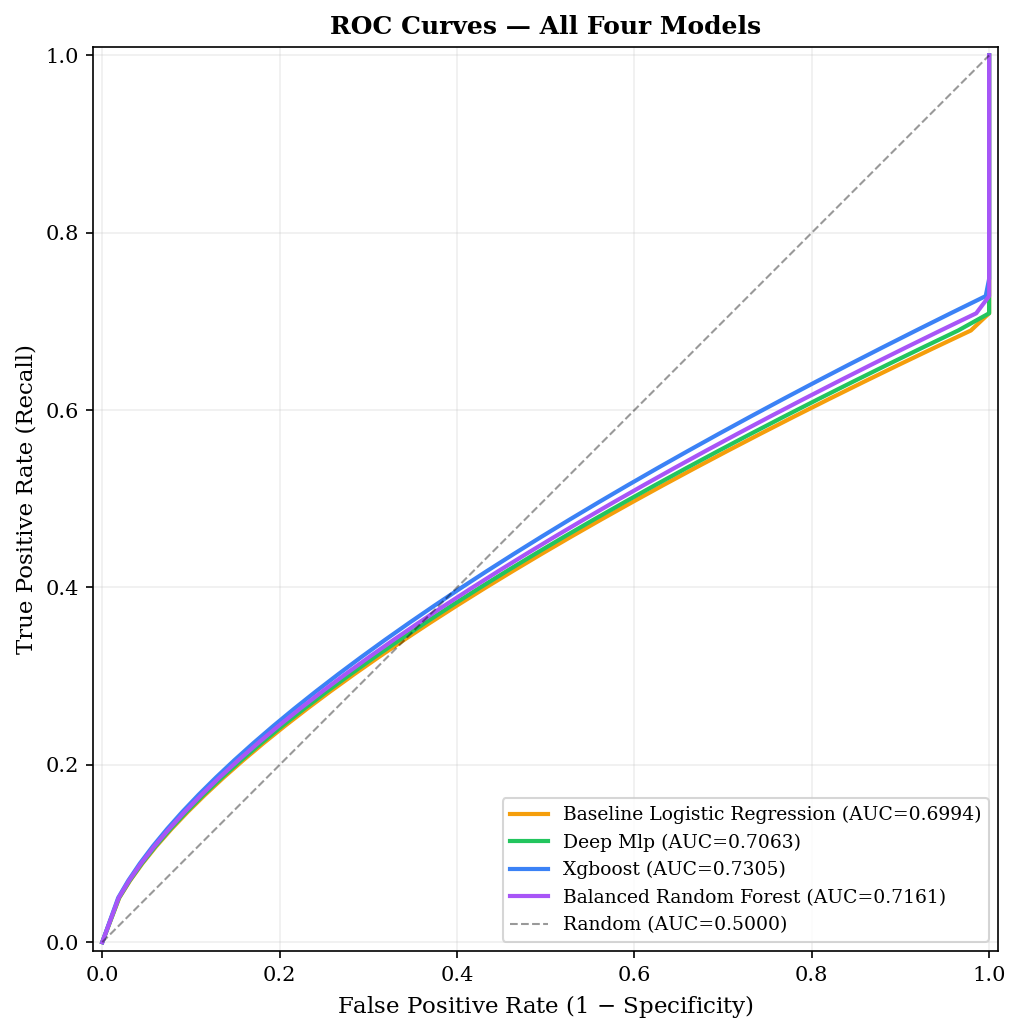
\includegraphics[width=0.85\textwidth]{report_figures/fig4_roc_curves.png}
\caption{ROC curves for all four ML models. XGBoost achieves best-in-class AUC of $0.7305$.}
\label{fig:roc}
\end{figure}

\begin{figure}[H]
\centering
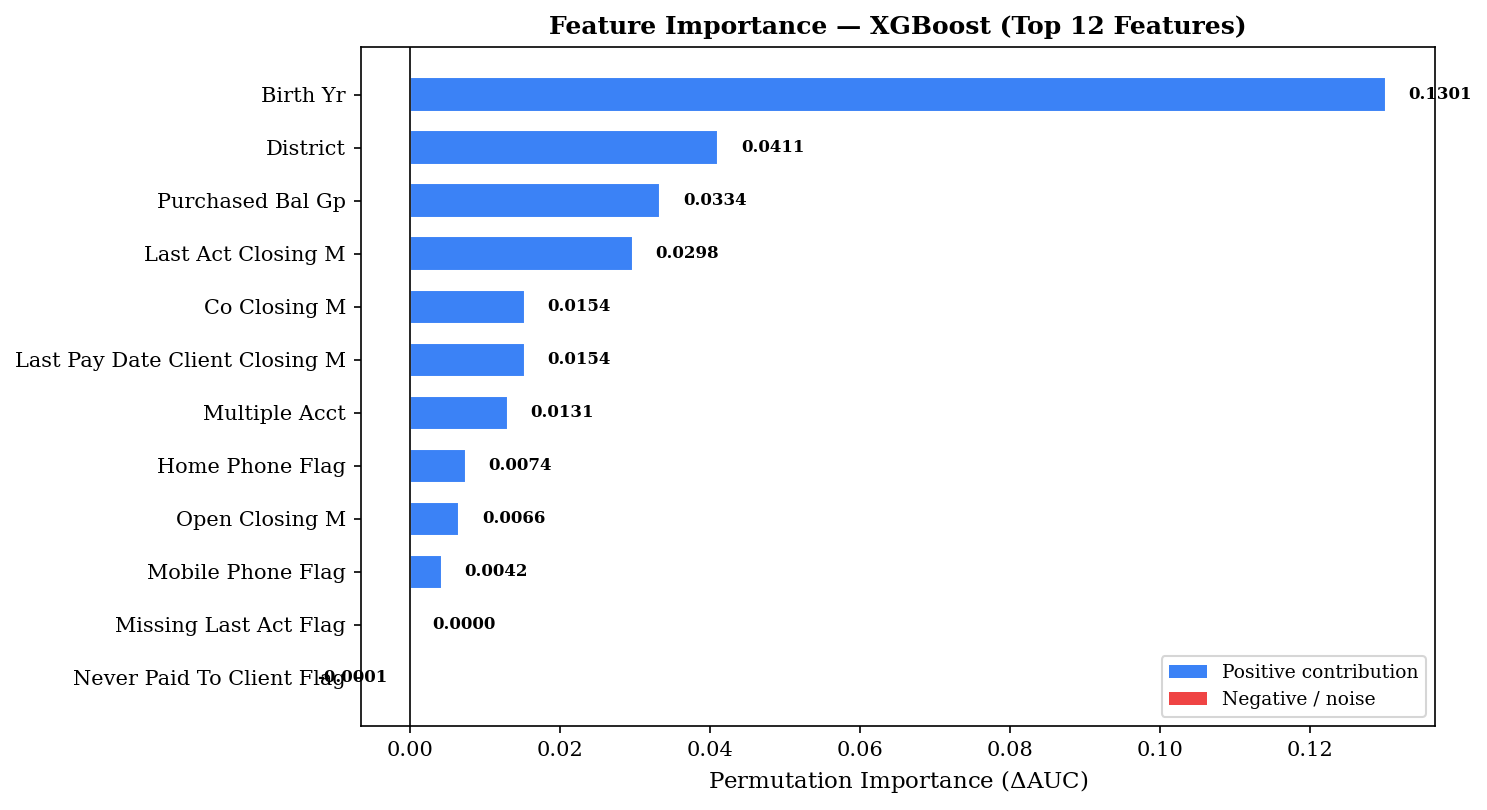
\includegraphics[width=0.88\textwidth]{report_figures/fig3_feature_importance.png}
\caption{Permutation importance for top 12 features (XGBoost champion). Birth year ($\Delta$AUC $=0.130$) dominates.}
\label{fig:fi}
\end{figure}

\begin{figure}[H]
\centering
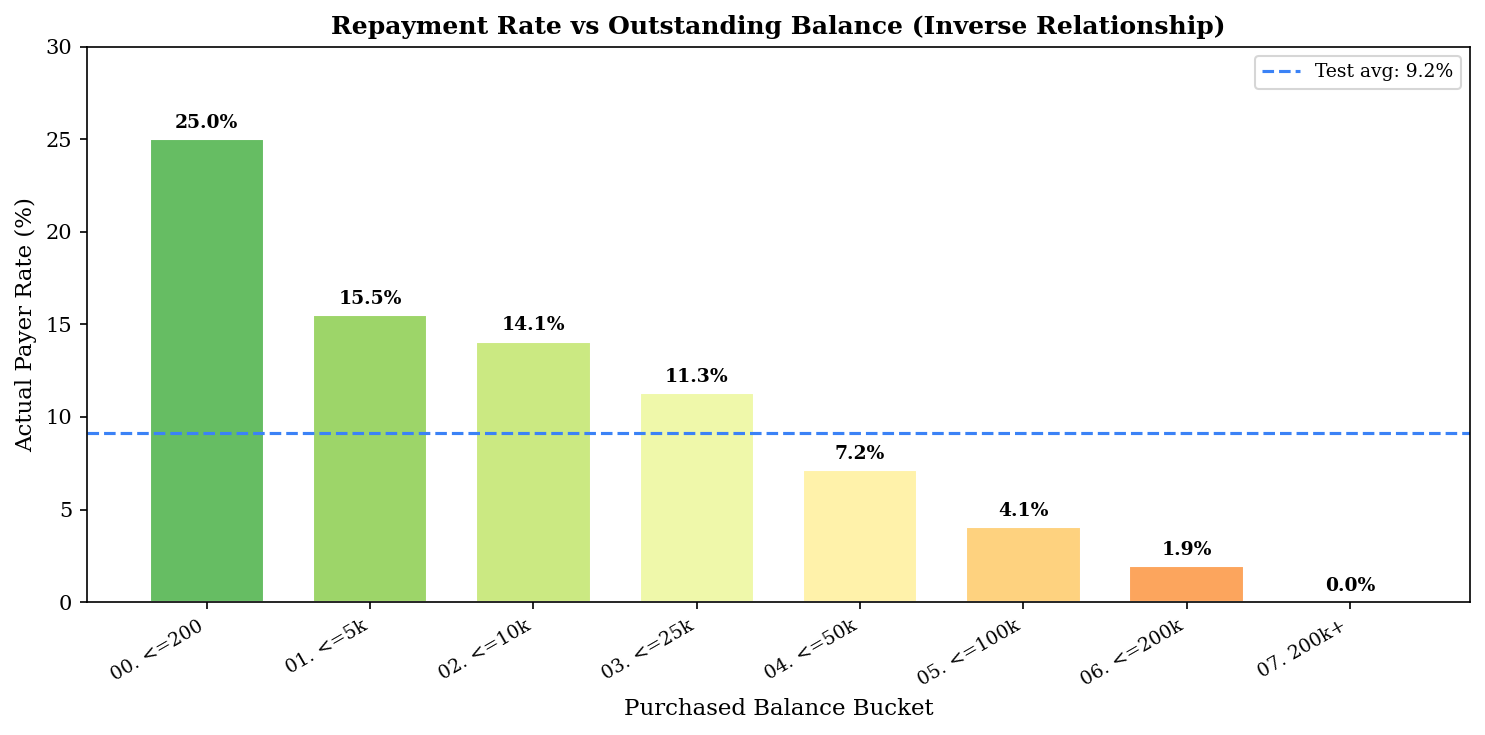
\includegraphics[width=0.78\textwidth]{report_figures/fig6_balance_payer_rate.png}
\caption{Actual payer rate by balance bucket. Dashed line $=$ test-set average ($9.15\%$). Inverse balance--repayment relationship.}
\label{fig:balance}
\end{figure}

\begin{figure}[H]
\centering
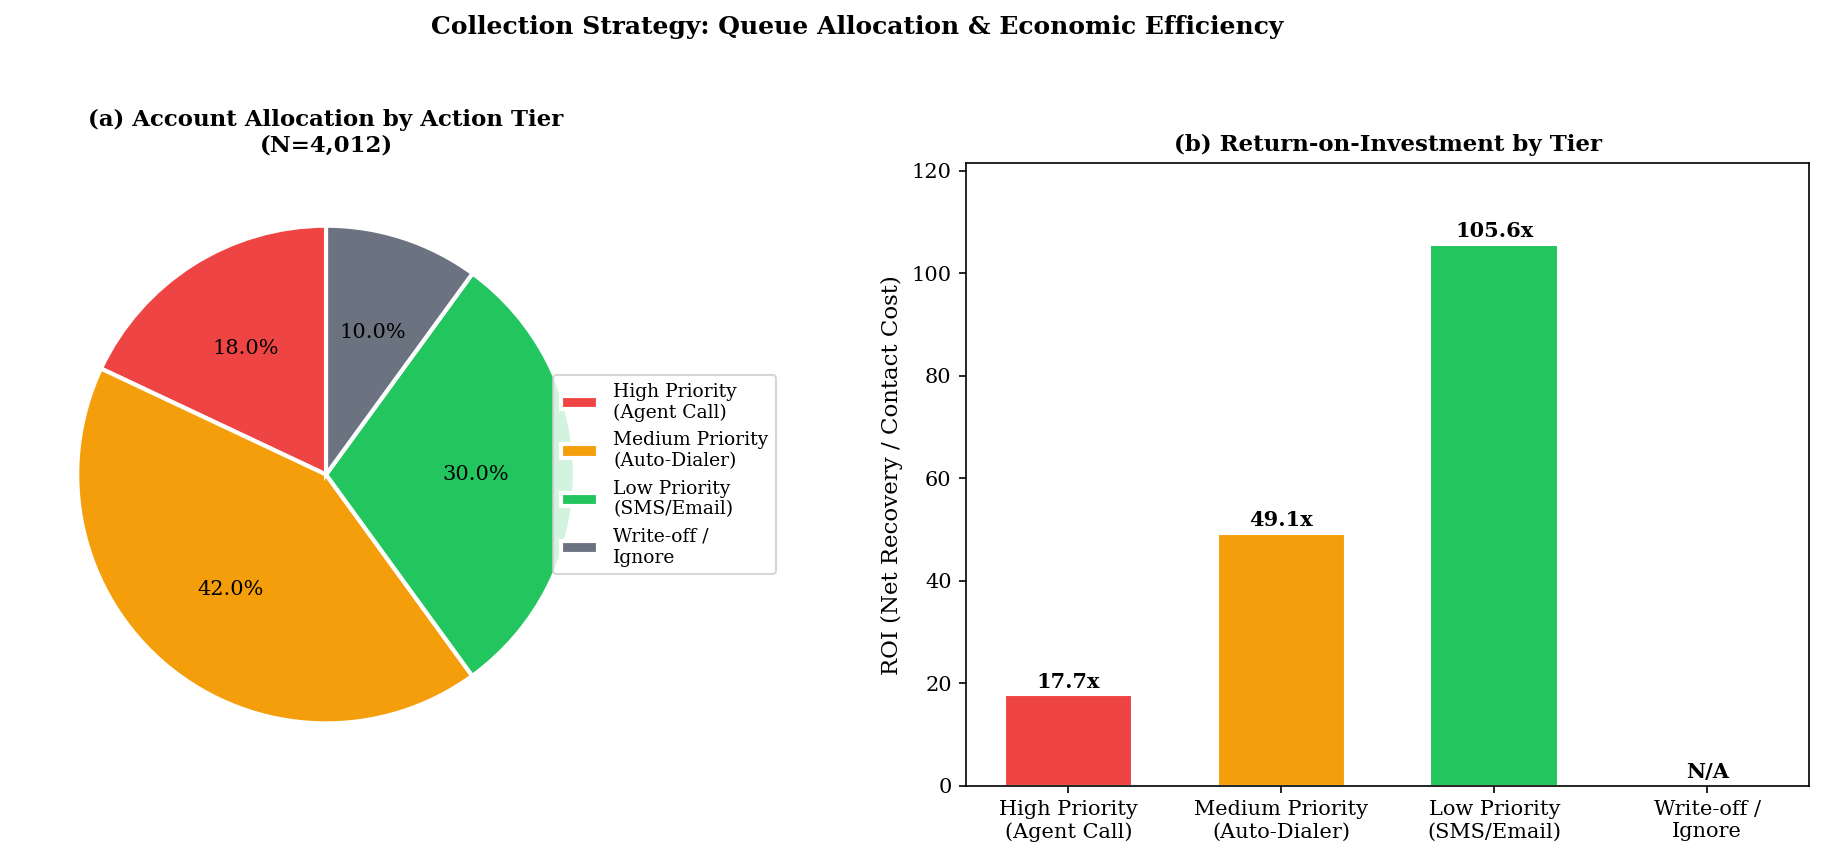
\includegraphics[width=0.85\textwidth]{report_figures/fig5_queue_allocation.png}
\caption{Optimized queue allocation. Top 20\% of accounts capture 50.6\% of expected net recovery.}
\label{fig:queue}
\end{figure}

\begin{figure}[H]
\centering

\includegraphics[width=0.95\textwidth]{report_figures/fig12_llm_cost_benefit.png}
\caption{LLM cost--benefit view: API cost (USD) and latency (ms/account) plotted against AUC. ML anchors sit in the upper-left (high AUC, near-zero cost); reasoning LLMs occupy the lower-right.}
\label{fig:llm_cost}
\end{figure}

\begin{figure}[H]
\centering
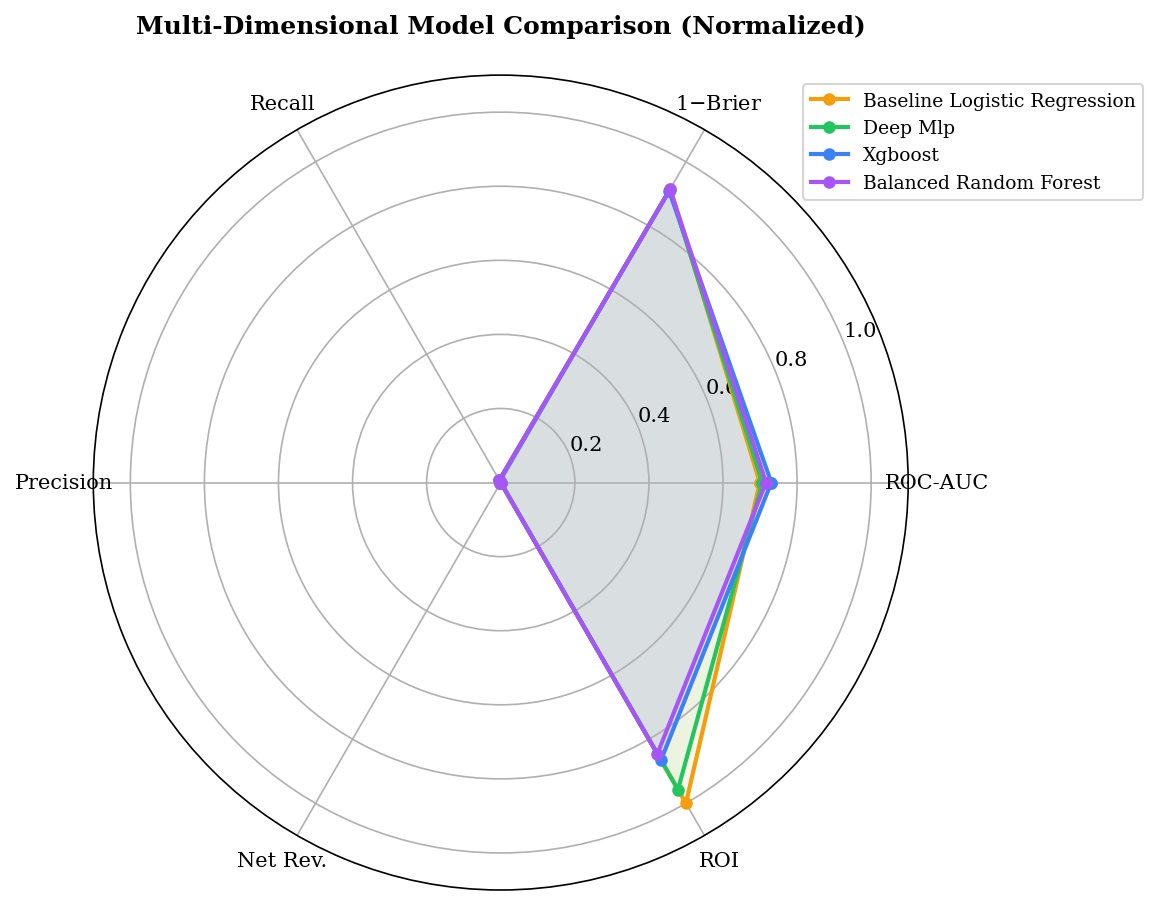
\includegraphics[width=0.7\textwidth]{report_figures/fig8_radar_chart.png}
\caption{Radar chart comparing all four ML models across six dimensions.}
\label{fig:radar}
\end{figure}

\begin{figure}[H]
\centering
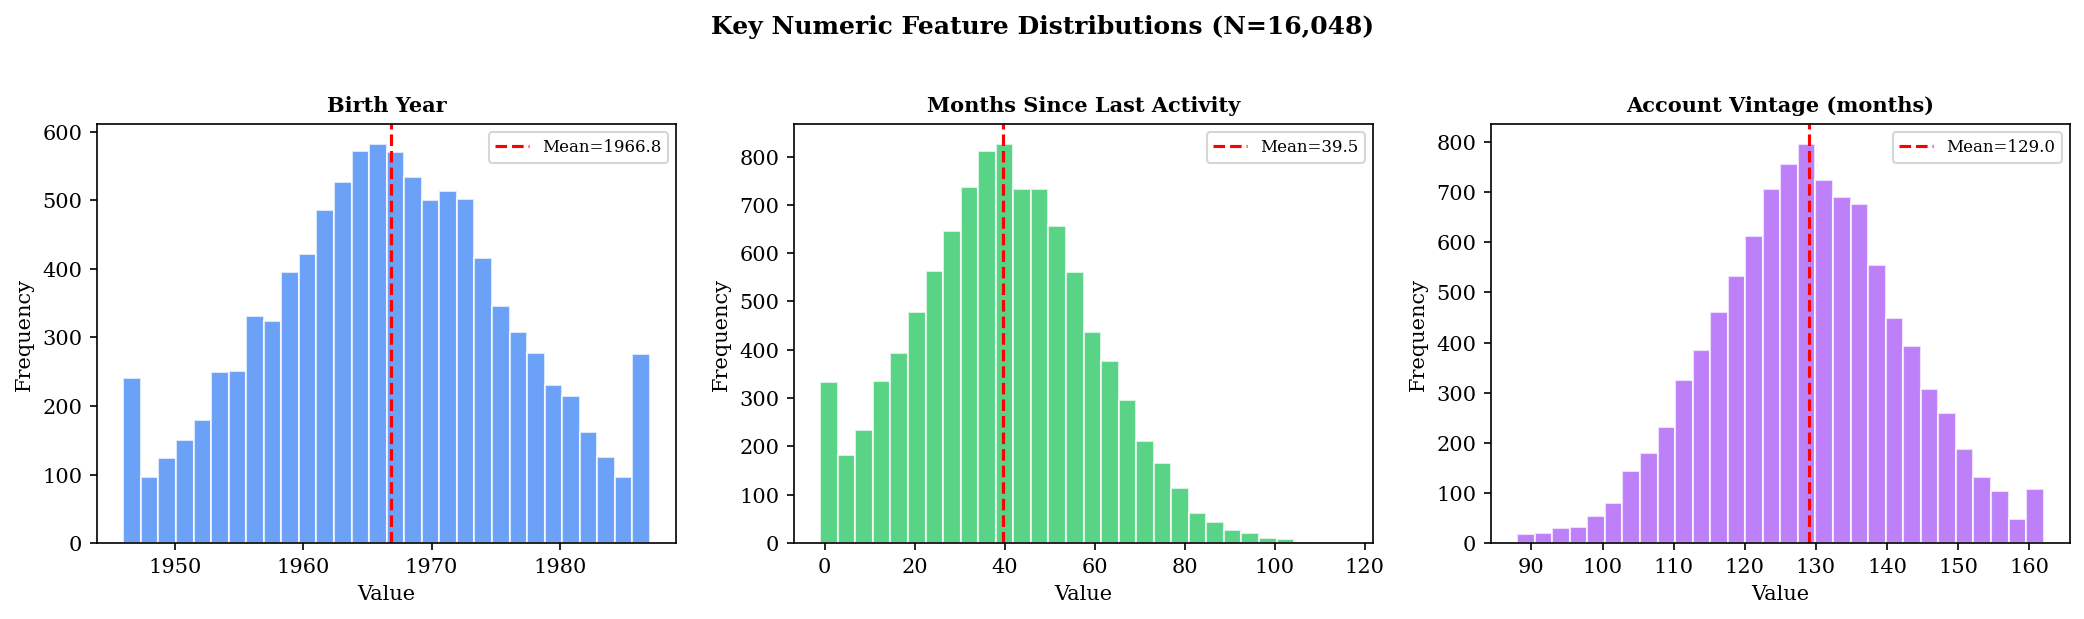
\includegraphics[width=\textwidth]{report_figures/fig7_distributions.png}
\caption{Distribution of three key numeric features ($N=16{,}048$).}
\label{fig:distributions}
\end{figure}

\end{document}
